\chapter{Utilizarea aplicației}

\section{Utilizator}
\subsection{Autentificarea}

Autentificarea reprezintă primul pas în utilizarea aplicației Voting App. Pentru a îmbunătății securitatea platformei, utilizatorilor nu le este permis să se înregistreze singuri, ei urmând să primească, atunci când le este creat contul de către un administrator, un mail pe adresa lor cu parola aferentă contului, parolă ce poate fi schimbată mai târziu, sau în cazul în care este uitată.

\begin{figure}[!ht]
    \centering
    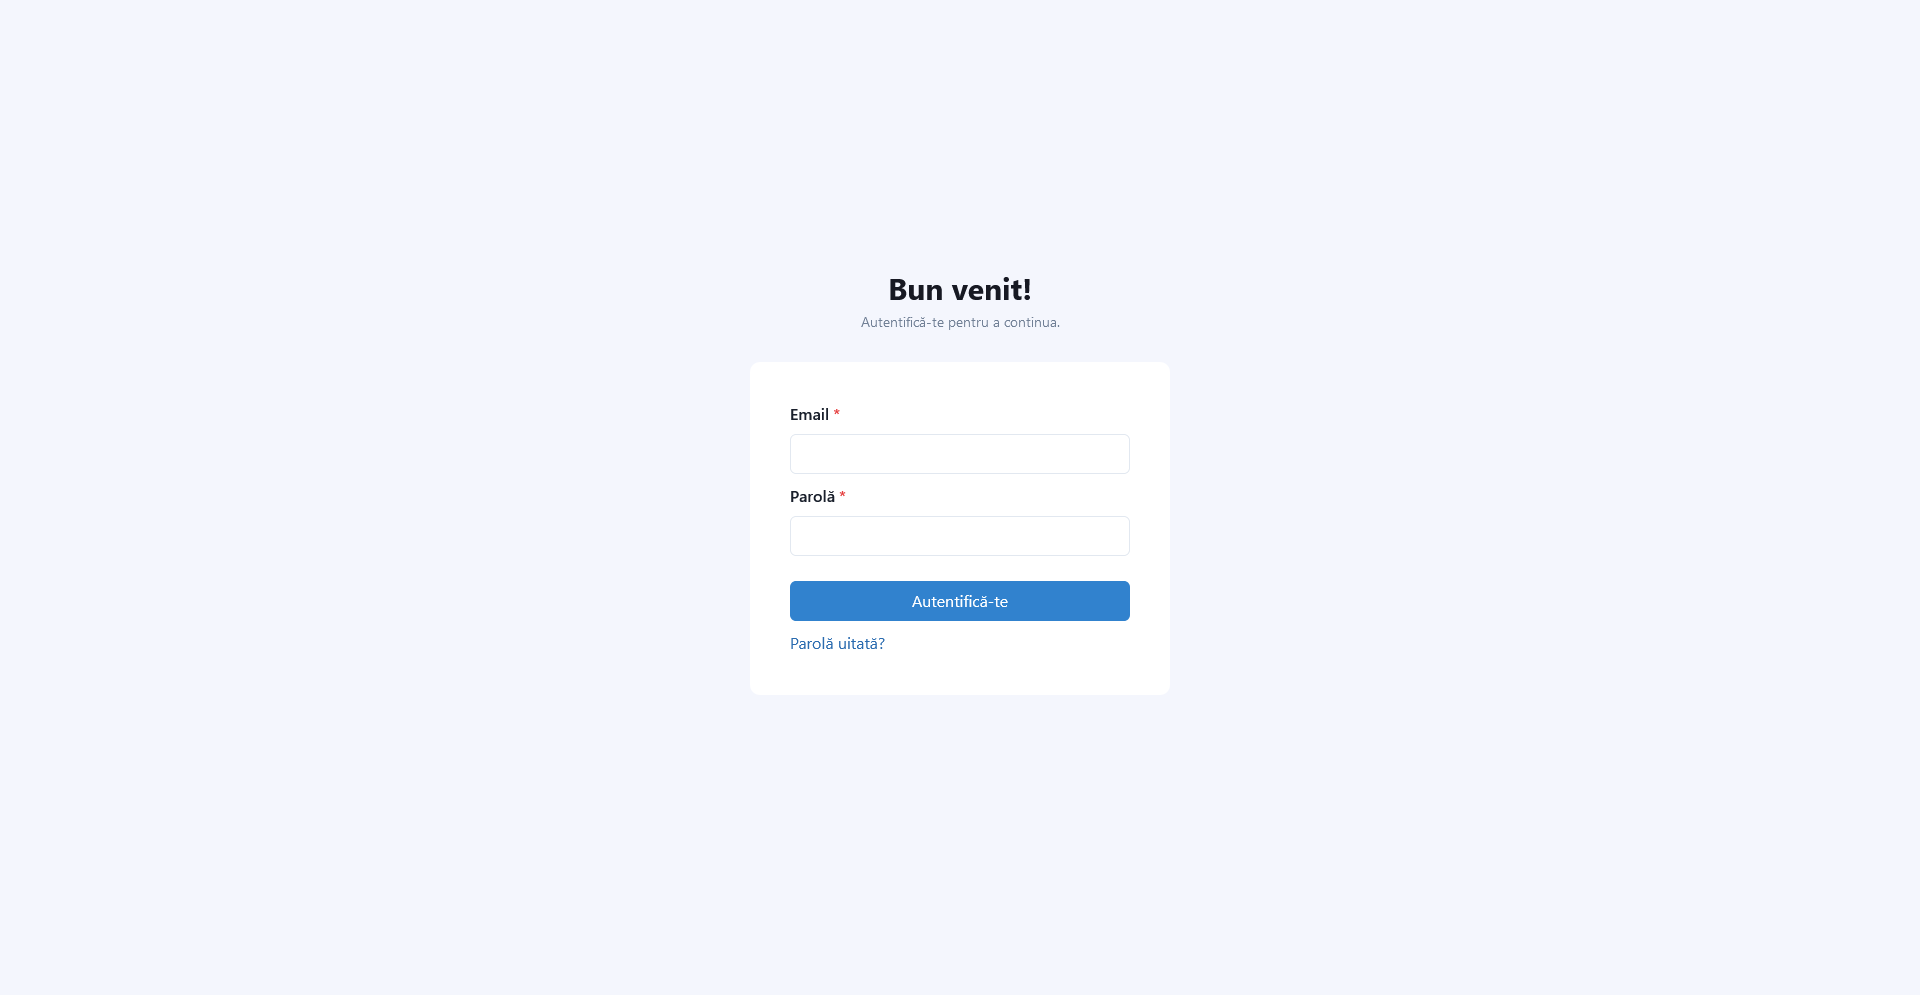
\includegraphics[width=145mm]{images/page_login.png}
    \caption{Captură a paginii de autentificare}
\end{figure}

\begin{figure}[!ht]
    \centering
    
\includegraphics[width=115mm]{images/example_mail_register.png}
    \caption{Exemplu de mail primit atunci când este creat un cont nou}
\end{figure}

\subsection{Meniul principal}

Meniul principal reprezintă punctul de start al aplicației și locul în care se va desfășura cea mai mare parte a unui utilizator pe platformă. Acesta conține datele utilizatorului și ultimele procese electorale în care acesta a fost inclus. De asemenea, conținutul tuturor paginilor este înfășurat în componenta \enquote{Layout}. Pentru a oferi o experiență cât mai plăcută și mai rapidă, a fost realizat un design minimalist ce scoate în evidență punctele de interes.

\begin{figure}[!ht]
    \centering
    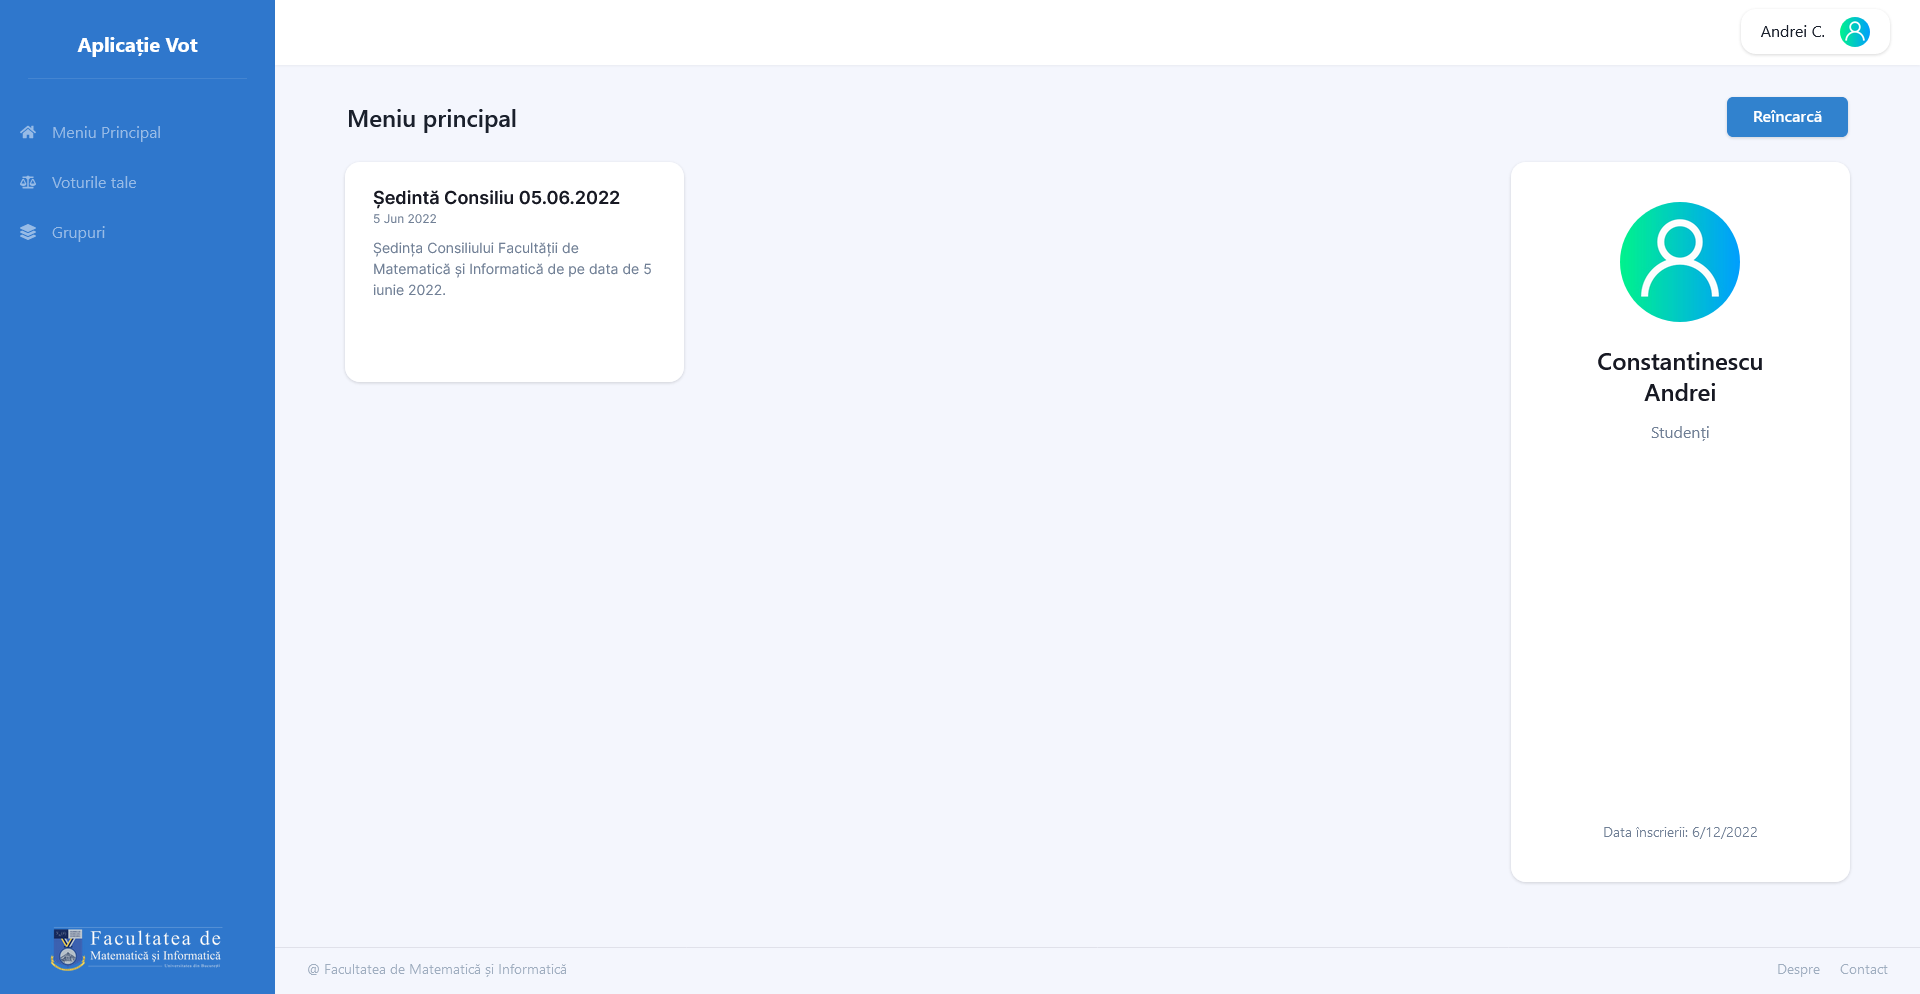
\includegraphics[width=145mm]{images/page_main.png}
    \caption{Captură a meniului principal}
\end{figure}

Componenta \enquote{Layout} conține, la rândul ei, alte patru componente: \enquote{Navbar}, \enquote{Sidebar}, \enquote{Titlebar} și \enquote{Footer}. În cazul în care utilizatorul este și administrator, componenta \enquote{Sidebar} va dispune de un buton suplimentar intitulat \enquote{Admin} ce va redirecționa utilizatorul către meniurile aferente.

\begin{figure}
\centering
\begin{subfigure}{.5\textwidth}
    \centering
    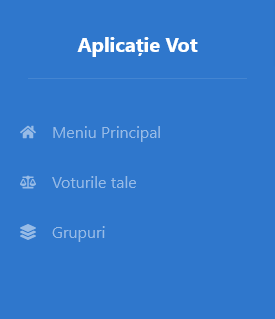
\includegraphics[width=45mm]{images/sidebar_normal.png}
\end{subfigure}%
\begin{subfigure}{.5\textwidth}
    \centering
    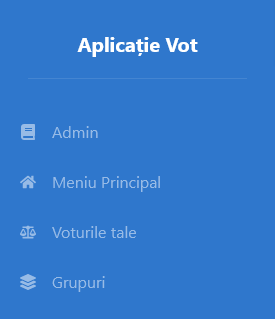
\includegraphics[width=45mm]{images/sidebar_admin.png}
\end{subfigure}
    \caption{Diferența componentei \enquote{Sidebar} între un utilizator și un administrator}
\end{figure}

\subsection{Pagini alternative}

Pe lângă meniul principal, utilizatorul mai are acces la câteva pagini:

\begin{itemize}
    \item \enquote{Voturile tale}. Aceasta conține totalitatea proceselor electorale la care utilizatorul a participat. Diferența dintre această pagina și meniul principal este lipsa cardului cu informațiile utilizatorului și prezența a absolut tuturor proceselor electorale, nu numai cele recente (prin recente se înțelege ultimele nouă procese electorale).
    \item \enquote{Grupuri}. Prezintă toate grupurile existente de pe platformă, astfel încât, în urma accesării unuia dintre grupuri, utilizatorul să primească detaliile aferente - nume, descriere, culoare și utilizatorii care fac parte din acel grup.
    \item \enquote{Setări}. Are o singură funcționalitate - conține un formular prin care utilizatorul își poate schimba parola contului.
\end{itemize}

\begin{figure}[!ht]
    \centering
    
\includegraphics[width=65mm]{images/settings_button.png}
    \caption{Accesarea pagini \enquote{Setări} se realizează prin butonul din componenta \enquote{Navbar}}
\end{figure}

\subsection{Procesul de votare}

Atunci când un nou proces electoral este creat, un nou cartonaș ce conține numele și descrierea votului va apărea pe meniul principal, iar, pentru a accesa chestionarul de votare, este necesară doar o simplă apăsare pe cartonaș.

\begin{figure}[!ht]
    \centering
    
\includegraphics[width=95mm]{images/cartonas_vot.png}
    \caption{Exemplu de cartonaș de vot}
\end{figure}

Imediat după accesare, utilizatorul va primi buletinul de vot unde își poate exprima opțiunile. De asemenea, în Voting App este implementată validarea datelor astfel încât să fie respectate cerințele unei întrebări, de exemplu numărul maxim sau numărul minim de opțiuni necesare unei selecții multiple. Butonul de \enquote{submit} va fi activat doar când formularul este valid.

\begin{figure}[!ht]
    \centering
    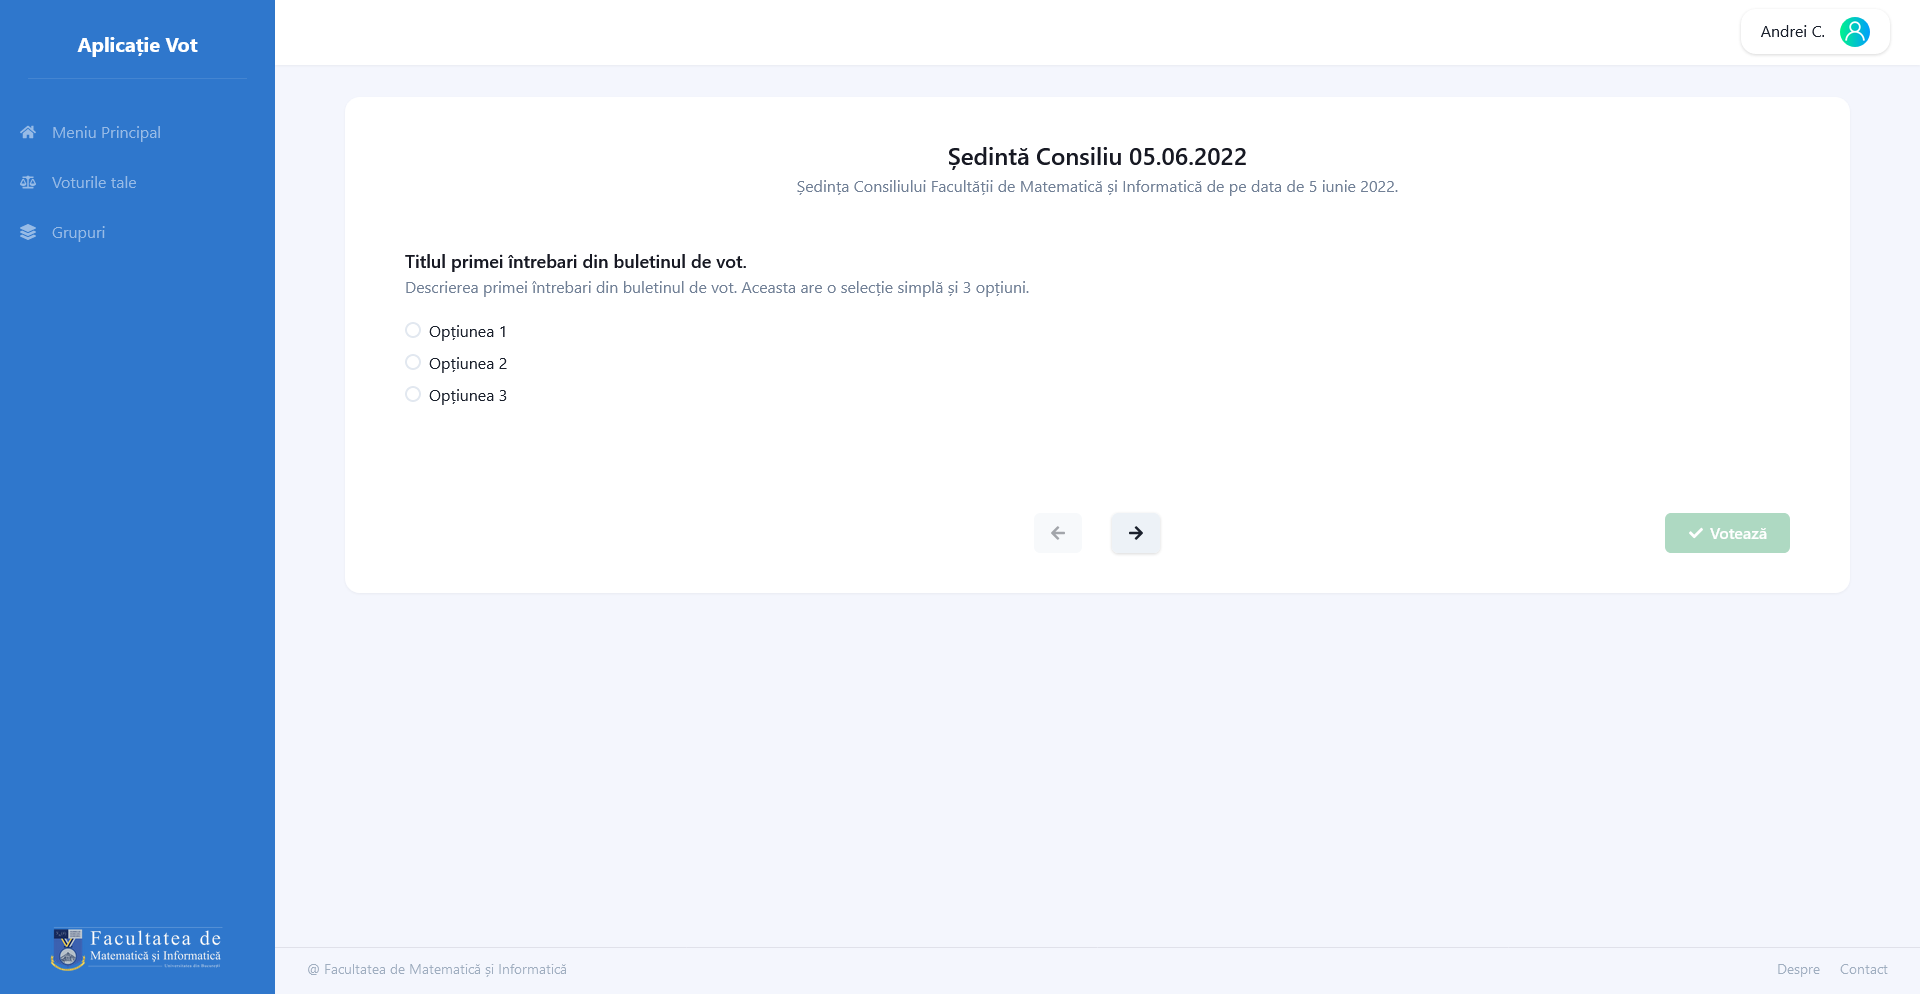
\includegraphics[width=145mm]{images/page_vote.png}
    \caption{Exemplu de buletin de vot, fiind prezentată prima întrebare din cele 2 date drept exemplu}
\end{figure}

\begin{figure}
\centering
\begin{subfigure}{.5\textwidth}
    \centering
    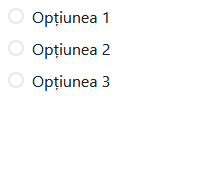
\includegraphics[width=45mm]{images/single_select.png}
\end{subfigure}%
\begin{subfigure}{.5\textwidth}
    \centering
    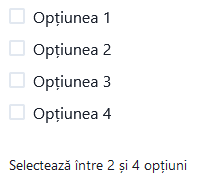
\includegraphics[width=45mm]{images/multiple_select.png}
\end{subfigure}
    \caption{Diferența între întrebările cu selecție simplă și cele cu selecție multiplă}
\end{figure}

În cadrul unui buletin de vot, utilizatorului îi pot fi adresate două tipuri de întrebări: cu selecție simplă, sau cu selecție multiplă. În cazul unei întrebări cu selecție simplă, utilizatorul poate alege numai una dintre opțiuni, pe când, în cazul unei întrebări cu selecție multiplă, utilizatorul poate alege mai multe opțiuni, fiind necesară încadrarea între un număr minim și un număr maxim de alegeri făcute.

Atunci când utilizatorul a completat toate chestionarele într-un mod corect, poate să își depună votul apăsând pe butonul \enquote{Votează}, unde va primi o notificare pe ecran pentru a confirma dacă este sigur de alegerea făcută. În urma confirmării și procesării de către aplicația de backend, acesta va fi redirecționat pe o pagină unde va apărea că votul lui a fost înregistrat. De asemenea, încercarea de a reaccesa formularul de vot va rezulta tot în afișarea mesajului de confirmare pentru a evita posibilitatea unei exprimări multiple a votului.

\begin{figure}[!ht]
    \centering
    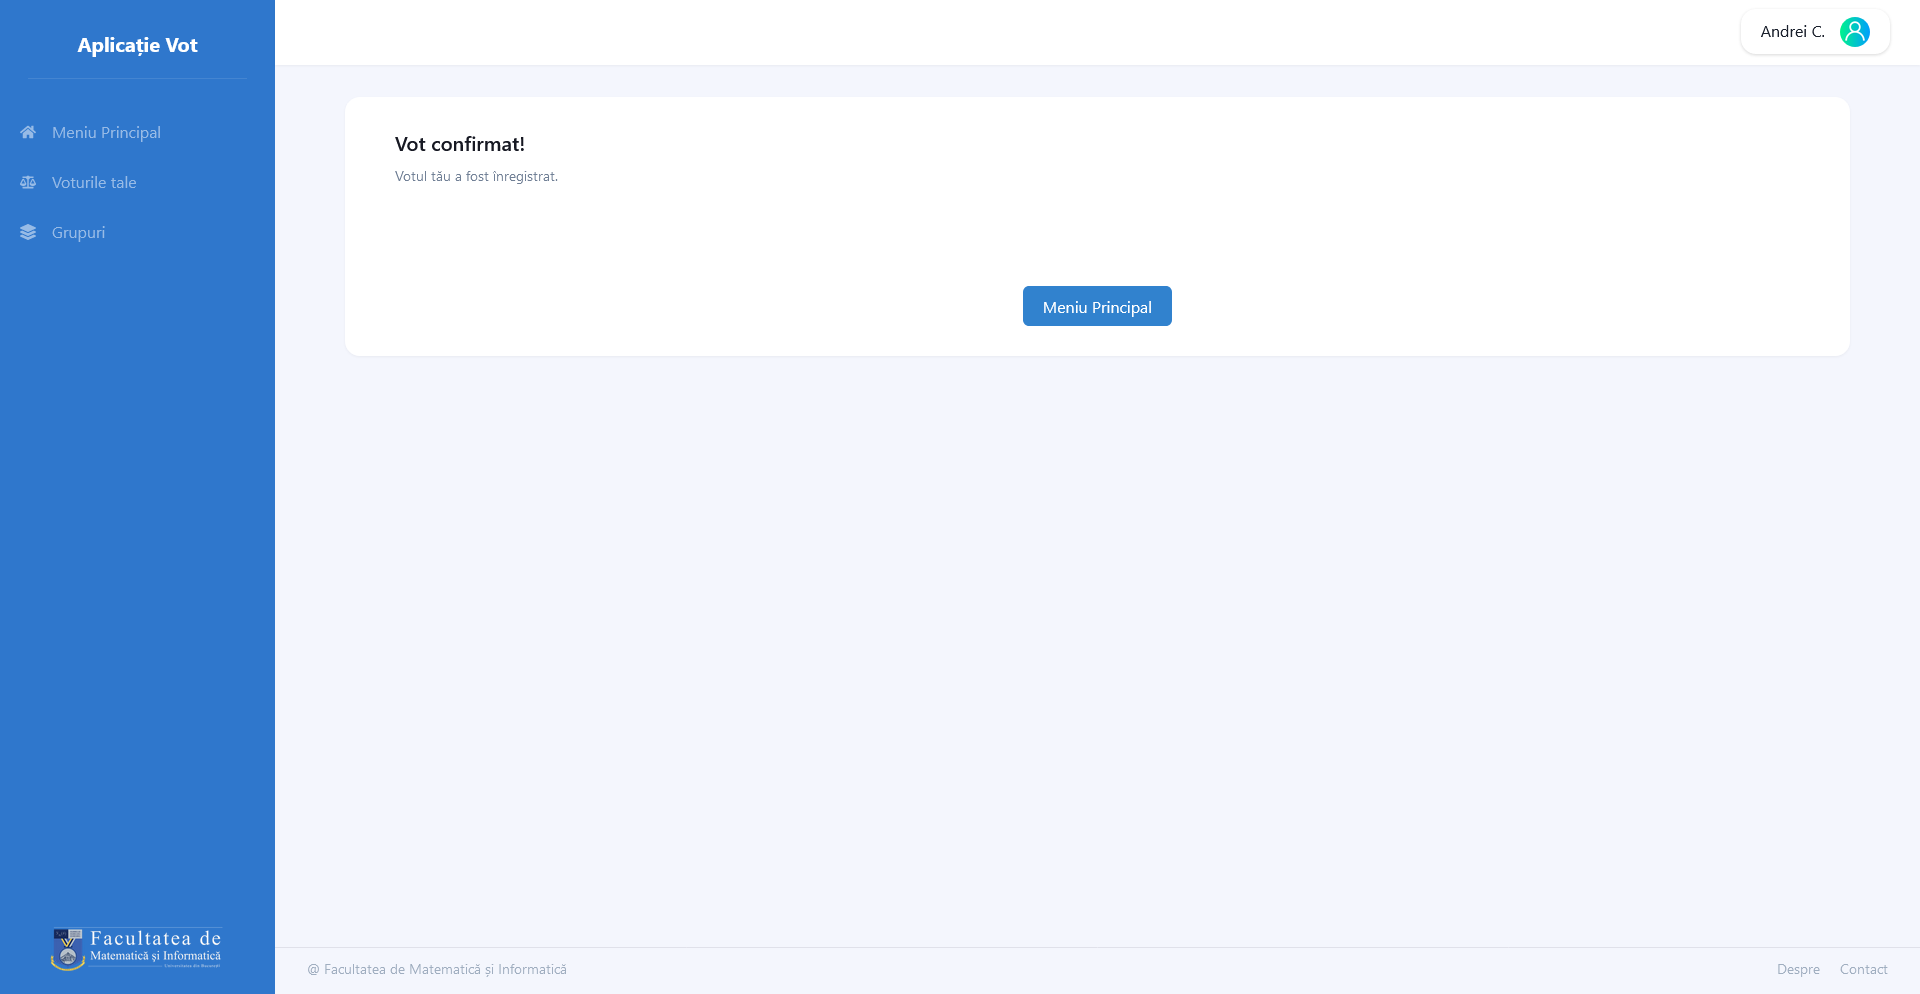
\includegraphics[width=145mm]{images/vote_confirmed.png}
    \caption{Captură a mesajului de confirmare}
\end{figure}

\subsection{Securitatea votului}

Deși HTTPS reprezintă un protocol securizat pentru transferul de date, aplicația Voting App adaugă un strat în plus de securitate atunci când vine vorba de încercarea înregistrării unui vot fals. Pentru a realiza acest lucru a fost implementată o funcție de \enquote{hash} ce are primește diverse date pentru a genera un cod de 256 de bits care este trimis spre aplicația de backend, odată cu finalizarea exprimării opțiunilor de vot, pentru a fi verificat. În cazul în care hash-ul nu este valid, votul depus nu o sa fie validat, astfel interceptând diverse încercări din afară de a falsifica voturi.

Funcția folosită pentru a genera hash-ul este SHA256, inventată în 2001 de către Agenția de Securitate Națională a Statelor Unite ale Americii și reprezintă, chiar și în ziua de azi, un standard în ceea ce înseamnă \enquote{hashing} \cite{what_is_hashing}. Deseori, acest algoritm este folosit pentru salvarea parolelor în bazele de date, astfel încât, în urma posibiltății unui atac cibernetic, atacatorii să nu aibă acces la parolele utilizatorilor, ci doar la hash-ul acestora.

\begin{code}
\begin{minted}[bgcolor=bg,frame=lines,framesep=2mm,fontsize=\footnotesize,baselinestretch=1]{js}
    // Preparing hash data
    const sent_on = new Date().toISOString();
    let hash = sha256(`${userSelector.id}.${params.id}.${sent_on}`);
\end{minted}
\captionof{figure}{Exemplu de cod pentru generarea hash-ului unui vot}
\label{code:hash-code}
\end{code}
\hfill

Securitatea algoritmului SHA256 este modelată de caracterul său ireversibil, dat fiind imposibilitatea realizării unui atac de tip \enquote{brute-force} într-un timp rezonabil, având la dispoziție nivelul tehnologic actual \cite{how_secure_sha}. În generarea unui hash, sunt utilizate atât funcții ireversibile, cât și de compresie, ce transformă datele de input. Un alt avantaj al folosirii acestui algoritm față de un altul este posibilitatea infimă de a întâmpina o coliziune - cazul în care două input-uri diferite rezultă în același output.

În aplicația Voting App, a fost folosit ca input al funcției SHA256 un string ce a rezultat din concatenarea identificatorului utilizatorului care și-a exprimat votul, identificatorului procesului electoral și data și ora exactă la care a fost depus votul, toate separate prin câte un punct. Rezultatul final va fi, întotdeauna, un șir de caractere de lungime 98.

\subsection{Schimbarea parolei}

Schimbarea parolei de către un utilizator se poate realiza în două moduri: prin formularul de la pagina setări, ce conține două câmpuri - unul pentru parola nouă și unul pentru confirmarea acesteia, sau prin formularul de \enquote{forgot password} prezent pe pagina de autentificare, în cazul uitării parolei.

Cel de al doilea formular implică trimiterea unui mail pe adresa utilizatorului. Acesta va conține un link către un formular de schimbare de parolă asemănător celui de la pagina "Setări". Ambele formulare necesită utilizatorului să introducă o parolă de minim opt caractere și care să conțină cel puțin o literă mare și un caracter special.

\begin{figure}[!ht]
    \centering
    
\includegraphics[width=135mm]{images/reset_pass_mail.png}
    \caption{Exemplu de mail pentru resetarea parolei}
\end{figure}

Mailurile sunt trimise folosind protocolul SMTP (Simple Mail Transfer Protocol) \cite{what_is_smtp}, integrat direct în framework-ul de backend. Textele mailurilor sunt generate dinamic, folosind datele utilizatorului care a făcut un request ce necesită trimiterea de mailuri.

De asemenea, este necesară crearea unei adrese de mail dedicate pentru a putea efectua transferul de mailuri și salvarea credențialelor acesteia în aplicația de backend. Pentru Voting App am folosit serviciul Gmail al Google, alături de funcționalitățile \enquote{two-factor authentification} și \enquote{app password} astfel încât trimiterea de mailuri să fie realizată direct, fără vreo altă aplicație terță.

\newpage

\section{Administrator}

\subsection{Meniul principal pentru administrator}

În urma autentificării cu un cont de administrator, utilizatorul va putea avea puteri sporite asupra aplicației, de exemplu să creeze și să șteargă conturi și grupuri, să creeze procese electorale și să le arhiveze. De asemenea, acesta decide când se va închide un proces electoral. Pentru a putea folosi toate aceste funcționalități, acesta dispune de un meniu principal care poate fi accesat din \enquote{Sidebar}, apăsând pe butonul \enquote{Admin}.

\begin{figure}[!ht]
    \centering
    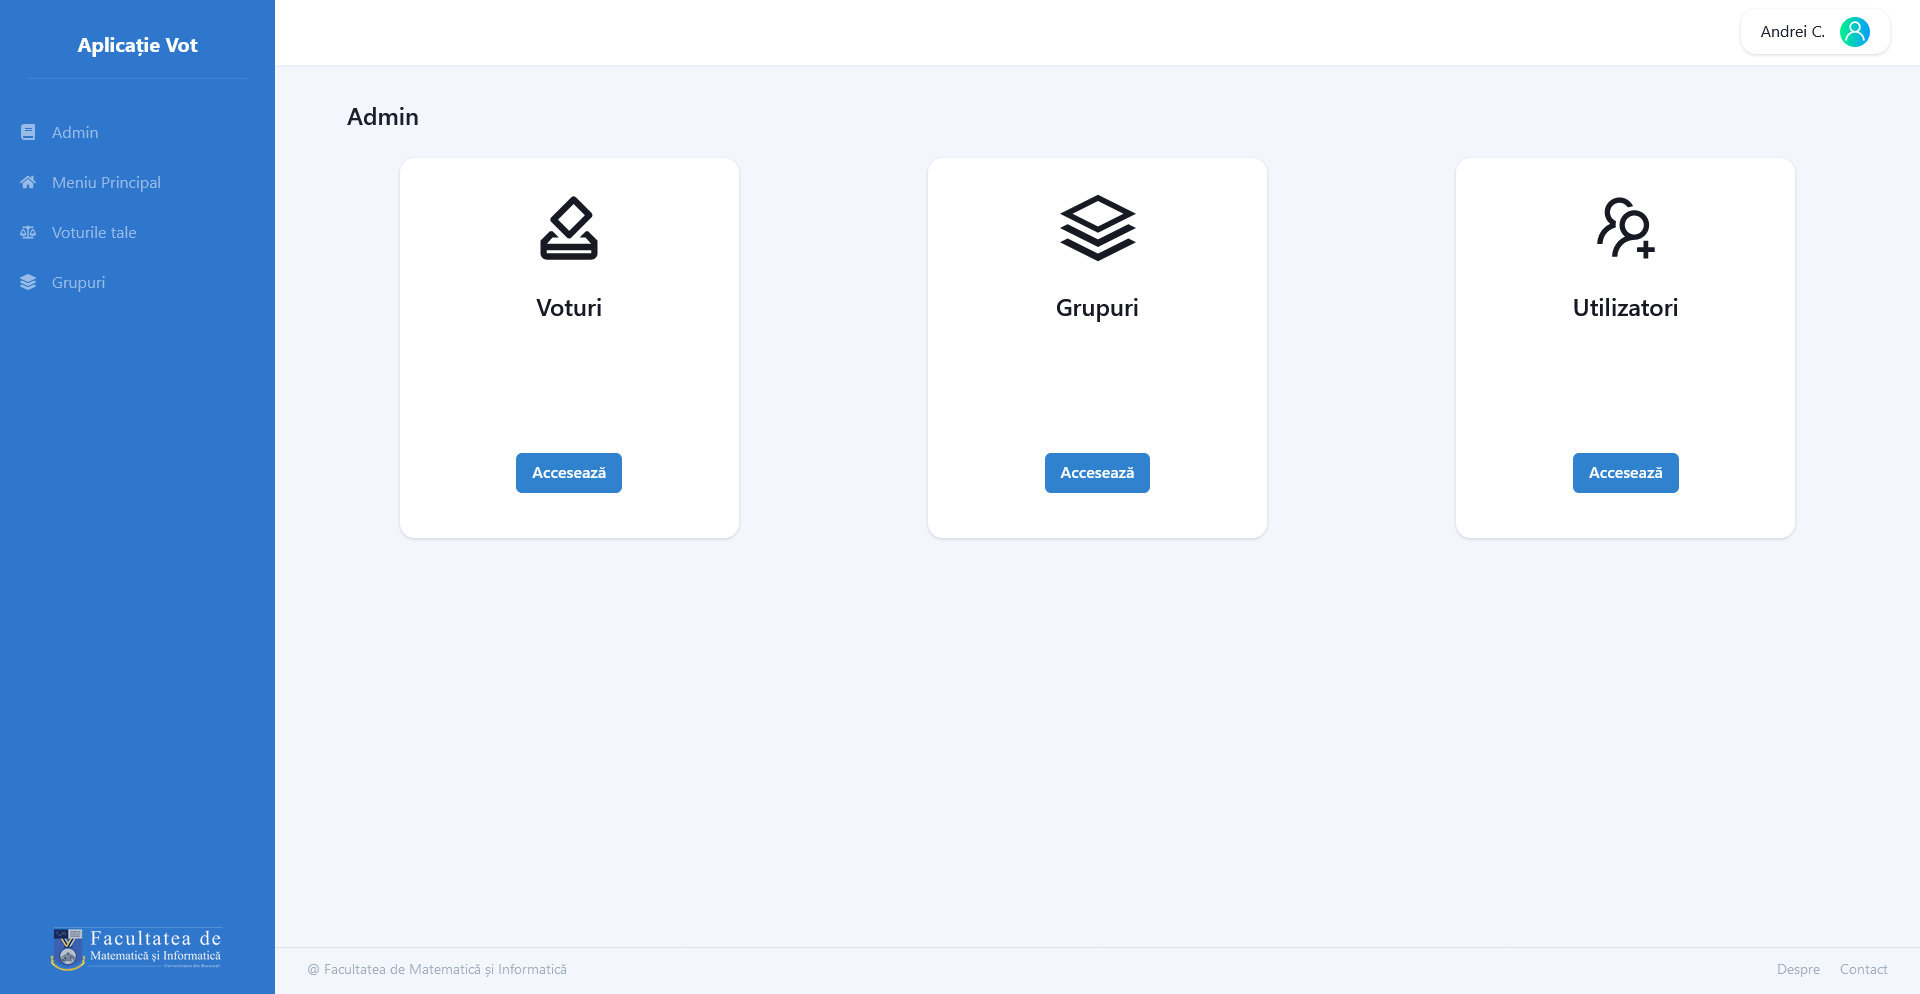
\includegraphics[width=135mm]{images/page_admin.png}
    \caption{Captură a meniului principal pentru administrator}
\end{figure}

Această pagină conține trei cartonașe ce permit administrarea rapidă și eficientă a platformei:

\begin{itemize}
    \item Cartonașul \enquote{Voturi}, conține formularul pentru a crea noi procese electorale și opțiunea de a le închide pe cele active.
    \item Cartonașul \enquote{Grupuri}, pentru a gestiona grupurile din platformă. Permite crearea, modificarea și ștergerea acestora.
    \item Cartonașul \enquote{Utilizatori}, folosit pentru a adăuga noi conturi pe platformă, a edita conturile active sau a le șterge pe cele inactive.
\end{itemize}

\newpage

\subsection{Crearea unui vot}

Primul cartonaș din meniul administratorului conține două tabele: cel pentru procesele electorale active și cel pentru procesele arhivate, accesat prin apăsarea butonului \enquote{Arhivă}. În dreptul fiecărui proces din listă se află un buton de \enquote{Detalii} ce va redirecționa administratorul în una din cele două opțiuni: în cazul unui proces electoral activ, pe pagina ce va arăta stadiul procesului, în direct, sau pe pagina de observare a rezultatului, în cazul unui proces încheiat și, implicit, arhivat. La baza tabelului din cadrul paginii de procese electorale active, se află butonul \enquote{Adaugă un vot}, menit pentru a redirecționa administratorul pe pagina ce conține formularul pentru crearea unui proces electoral.

Formularul de creare a unui vot reprezintă una dintre cele mai complexe funcționalități ale platformei, dat fiind caracterul lui dinamic. Pentru a crea un proces electoral, formularul a fost împărțit în trei segmente de bază:

\begin{itemize}
    \item Informații generale
    \item Grupuri
    \item Întrebări
\end{itemize}

Segmentul de informații generale conține două câmpuri: titlul buletinului de vot și descrierea acestuia. Aceste informații vor fi afișate pe toate paginile buletinului de vot.

Segmentul pentru grupuri este format dintr-o listă a tuturor grupurilor active pe platformă, unde administratorul poate selecta ce grupuri de utilizatori își vor exprima votul.

\begin{figure}[!ht]
    \centering
    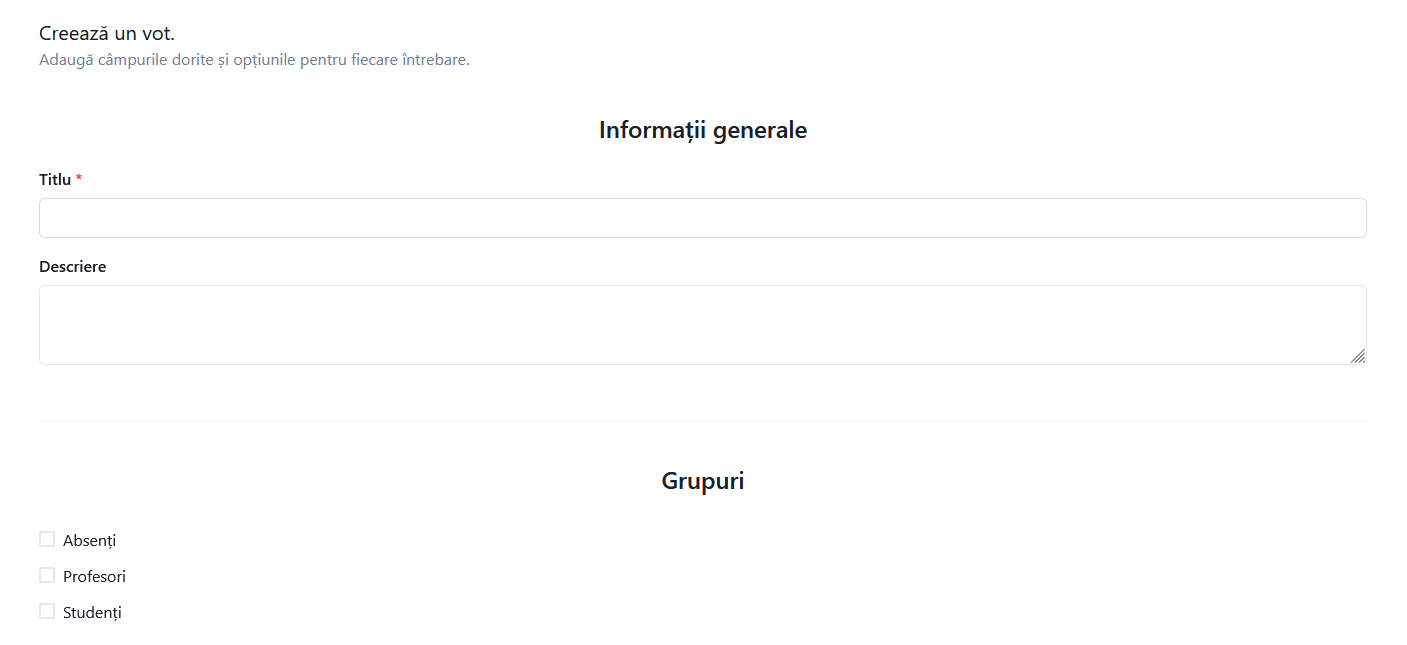
\includegraphics[width=145mm]{images/create_vote1.png}
    \caption{Segmentele \enquote{Informații generale} și \enquote{Grupuri}}
\end{figure}

Nu în ultimul rând, segmentul pentru întrebări conține o modalitate dinamică de generare a acestora și a opțiunilor aferente, similar funcționalității unui Google Form. Administratorul are de completat câmpurile pentru titlul și descrierea întrebării și de selectat tipul acesteia - selecție simplă sau selecție multiplă. În cazul în care administratorul decide să genereze o întrebare cu selecție multiplă acesta va fi nevoit să completeze câmpurile pentru selecții minime și selecții maxime. În cazul adăugării unei noi întrebări, acesta va apăsa butonul \enquote{Adaugă o întrebare}, iar în cazul ștergerii unei întrebări din listă, butonul \enquote{Șterge întrebarea}. Pentru fiecare întrebare, va fi nevoită generarea a cel puțin două opțiuni prin utilizarea câmpurilor aferente. Pentru a adăuga o opțiune, există butonul \enquote{Adaugă o opțiune}, iar pentru ștergere se va folosi butonul \enquote{X} din dreptul unei opțiuni.

\begin{figure}[!ht]
    \centering
    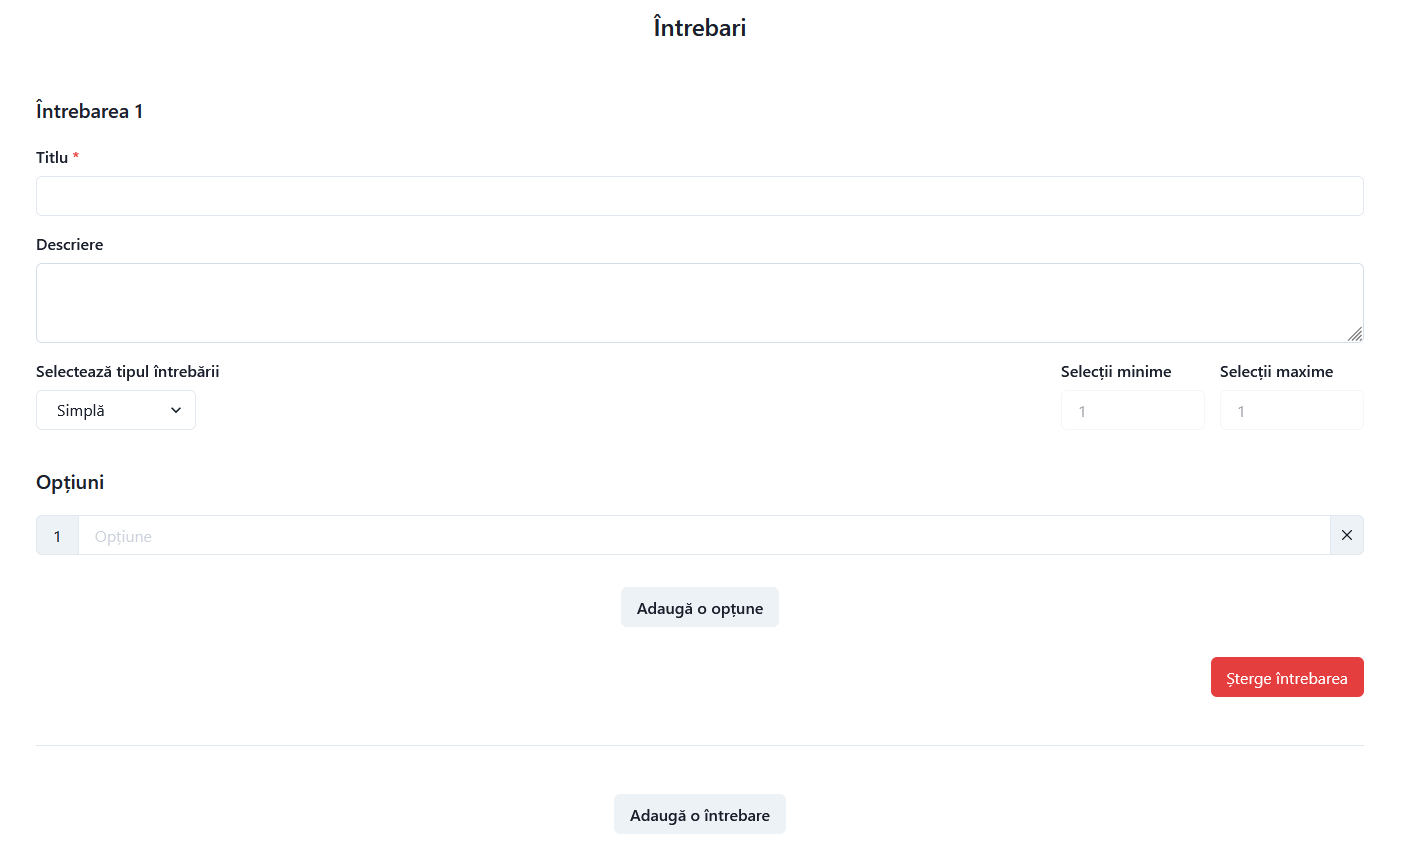
\includegraphics[width=135mm]{images/create_vote2.png}
    \caption{Segmentul \enquote{Întrebări}}
\end{figure}

Fiecare câmp din formular necesită validare, astfel, administratorul nu va putea genera un proces electoral dacă nu are toate câmpurile valide. Pentru fiecare câmp, chiar și cele create dinamic, va fi afișat un mesaj de avertizare în cazul în care acesta nu este valid.

Ultimul pas este reprezentat de apăsarea butonului \enquote{Finalizează} ce afișează administratorului un mesaj de confirmare. După confirmare, procesul electoral este început, iar utilizatorii își pot exprima votul.

\subsection{Încheierea unui proces electoral și observarea rezultatului}

Odată ce un proces electoral este creat, acesta va apărea în lista de procese electorale active din meniul "Voturi", unde, pentru fiecare proces în parte, există un buton \enquote{Detalii}, care va redirecționa administratorul către o pagină ce oferă statistici în direct asupra procesului electoral selectat. Pe această pagină apar informații despre stadiul actual, printre care: numărul total de votanți, numărul de votanți care și-au exprimat votul și lista acestora și butonul "Stop Vot". Atunci când expiră timpul de votare, sau administratorul decide să încheie votul, acesta va apăsa butonul pentru oprire și va fi redirecționat către pagina care va afișa rezultatul procesului electoral.

\begin{figure}[!ht]
    \centering
    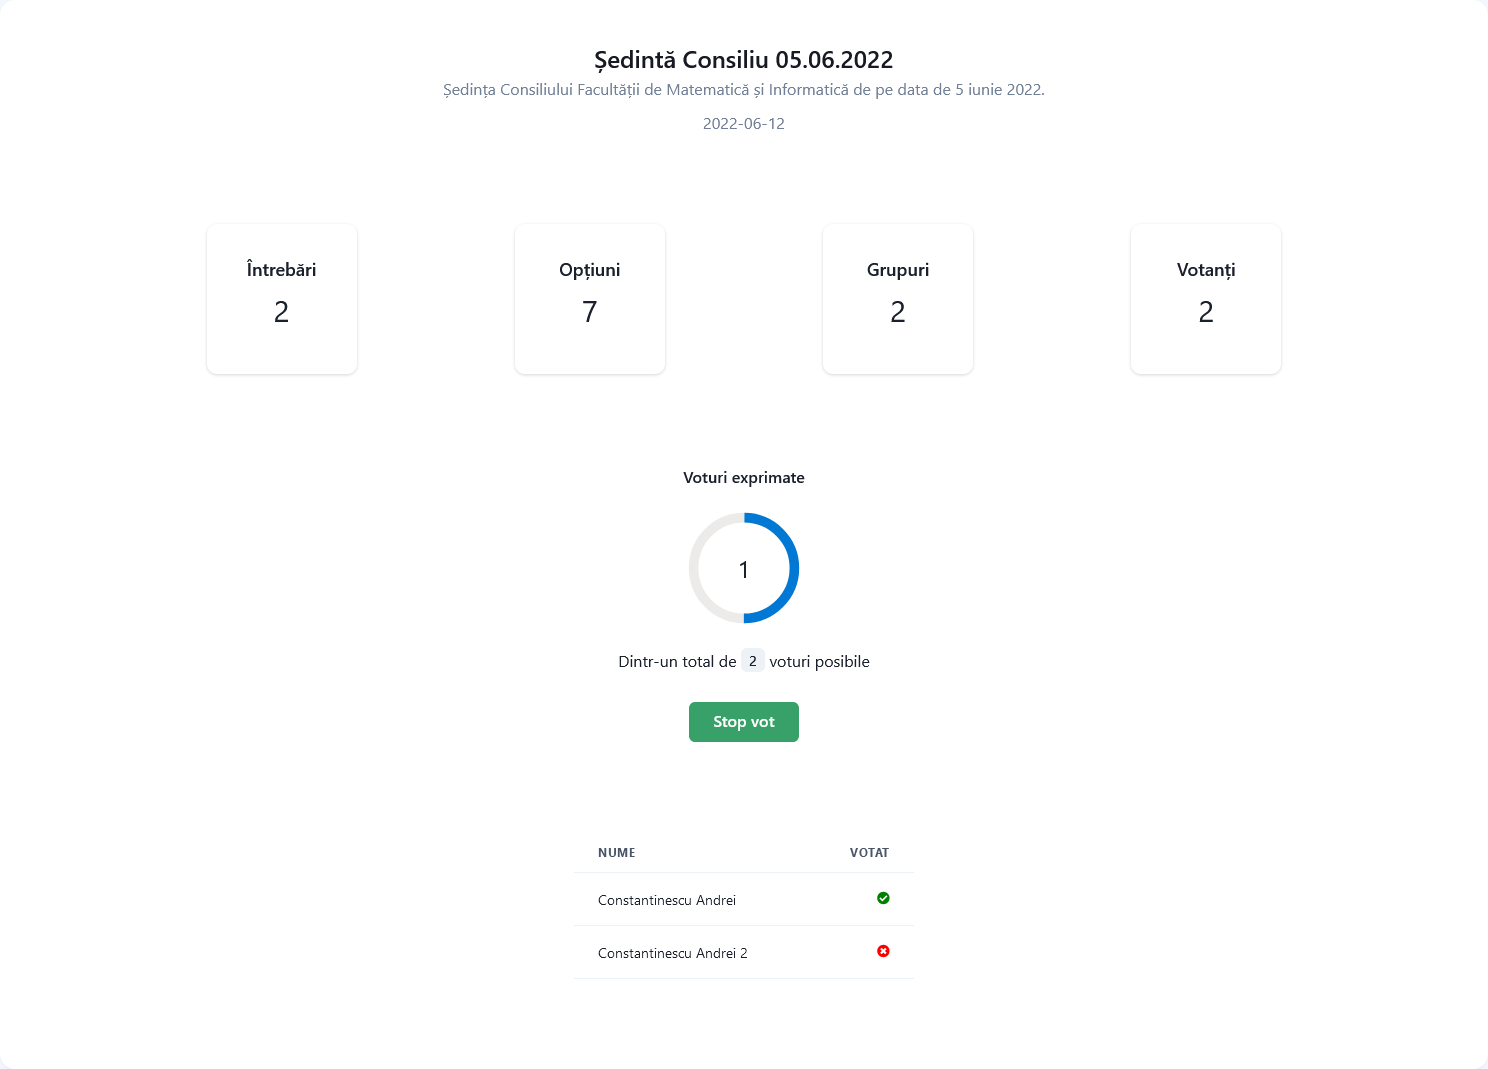
\includegraphics[width=135mm]{images/example_vote_details.png}
    \caption{Exemplu de detalii ale unui proces electoral}
\end{figure}

Pe pagina generată pentru observarea rezultatelor, vor fi afișate toate întrebările din buletinul de vot, fiecare cu opțiunile aferente și, în dreptul fiecărei dintre opțiuni, numărul de voturi exprimate în favoarea ei. În cazul în care o opțiune a unei întrebări reușește să strângă 50\% + 1 din voturi, aceasta va fi scoasă în evidență.

\begin{figure}[!ht]
    \centering
    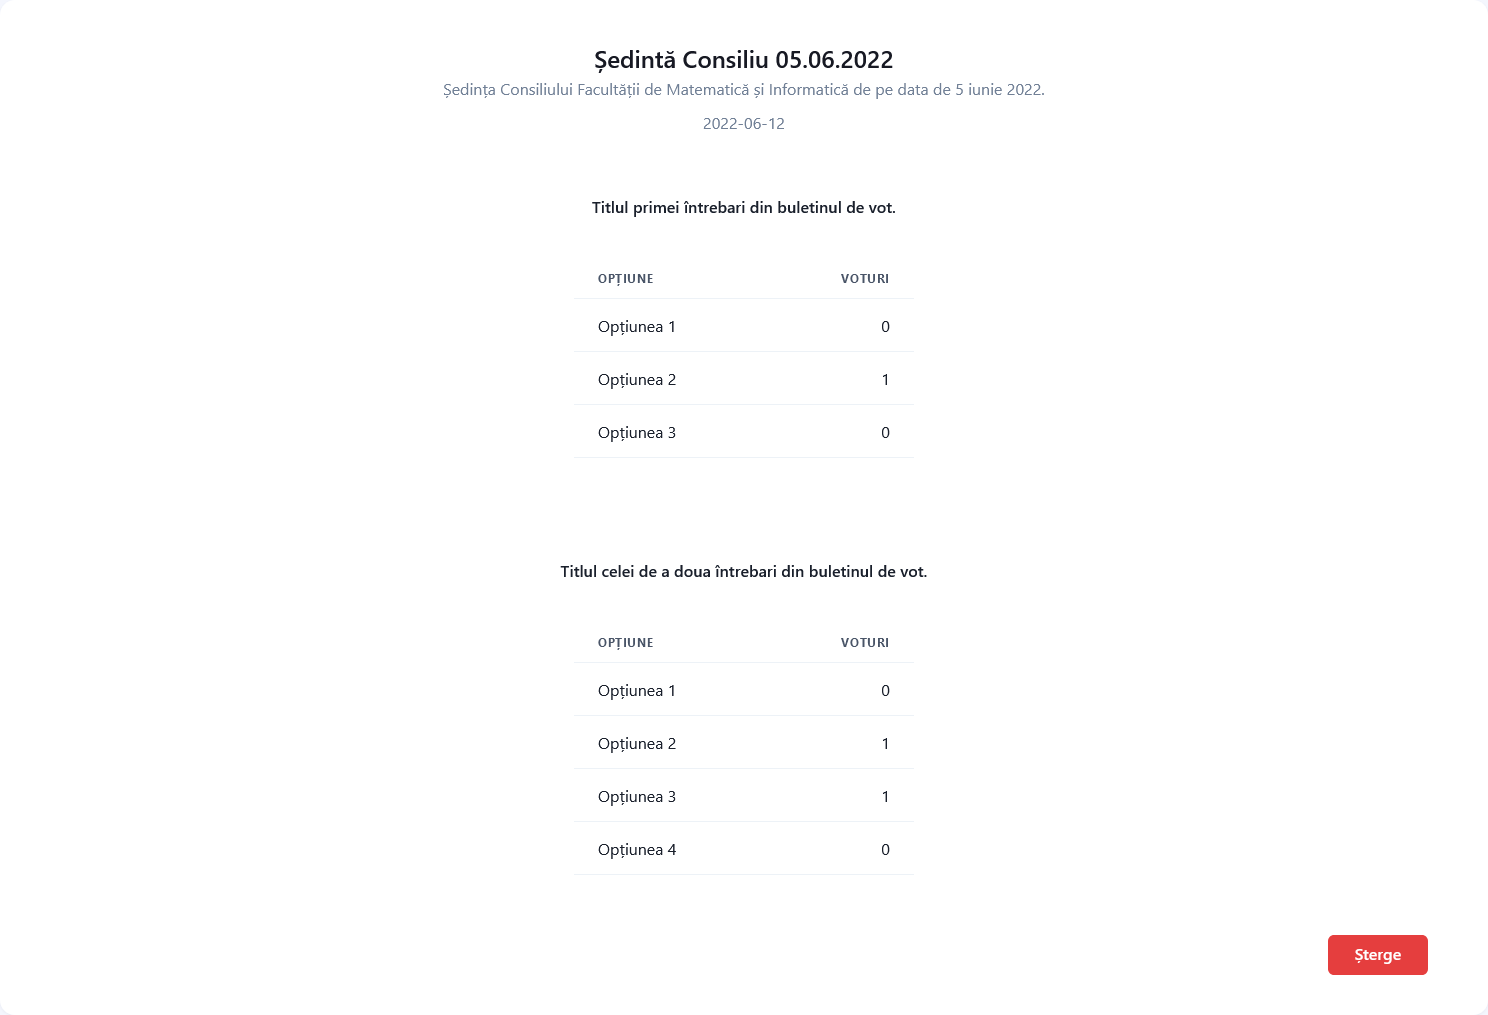
\includegraphics[width=135mm]{images/example_vote_results.png}
    \caption{Exemplu de rezultat al unui proces electoral încheiat}
\end{figure}

\newpage

\subsection{Operații de tip CRUD pe utilizatori și grupuri}

Următoarele două cartonașe din panoul de administrator sunt folosite pentru a accesa meniurile aferente operațiilor de creare, editare și ștergere atât a grupurilor, cât și a utilizatorilor. Ca funcționalitate, cele două se aseamănă, ambele conținând un formular ce se poate regăsi în două \enquote{state-uri} diferite - necompletat, în cazul creării unui cont de utilizator nou sau a unui grup nou, sau deja completat, caz în care valorile inițiale ale formularului vor conține datele aferente grupului sau utilizatorului ales. De asemenea, toate câmpurile din cele două formulare trebuie să fie valide pentru a putea continua.

\begin{figure}[!ht]
    \centering
    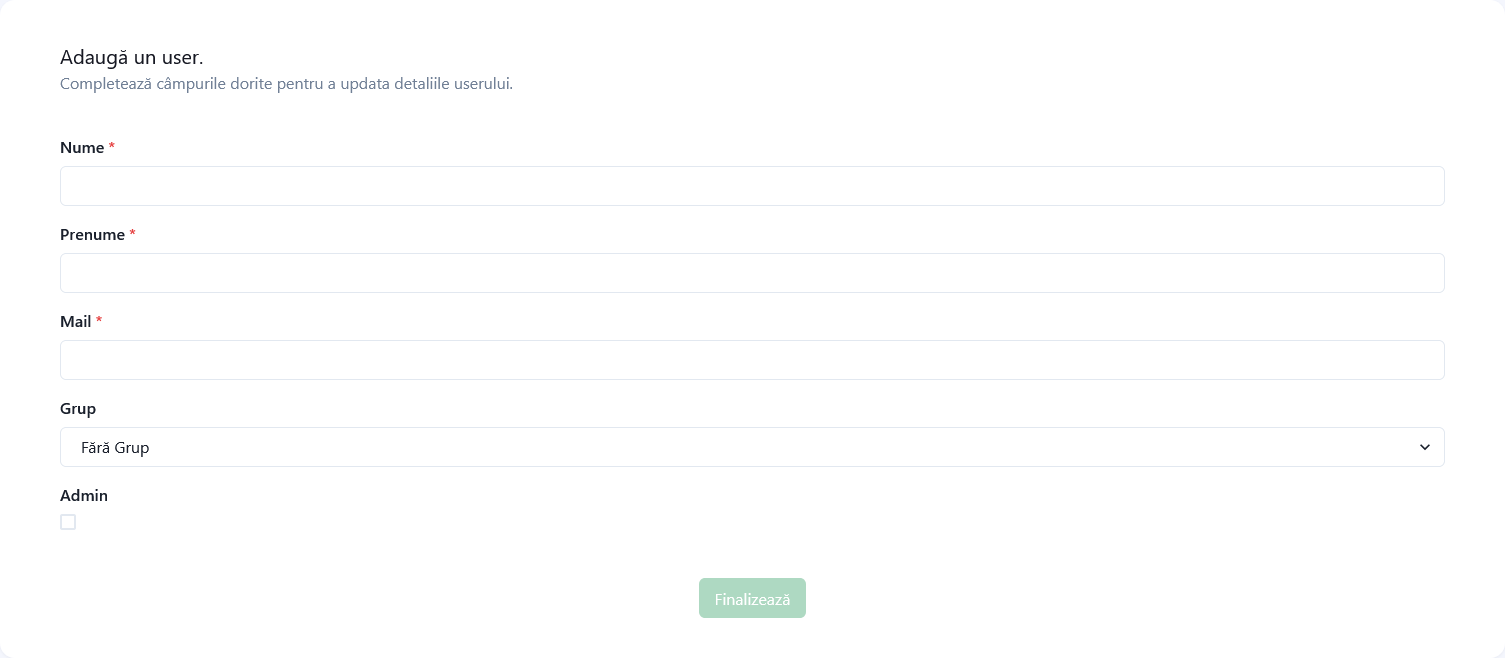
\includegraphics[width=140mm]{images/crud_user.png}
    \caption{Formularul pentru crearea unui cont de utilizator}
\end{figure}

\begin{figure}[!ht]
    \centering
    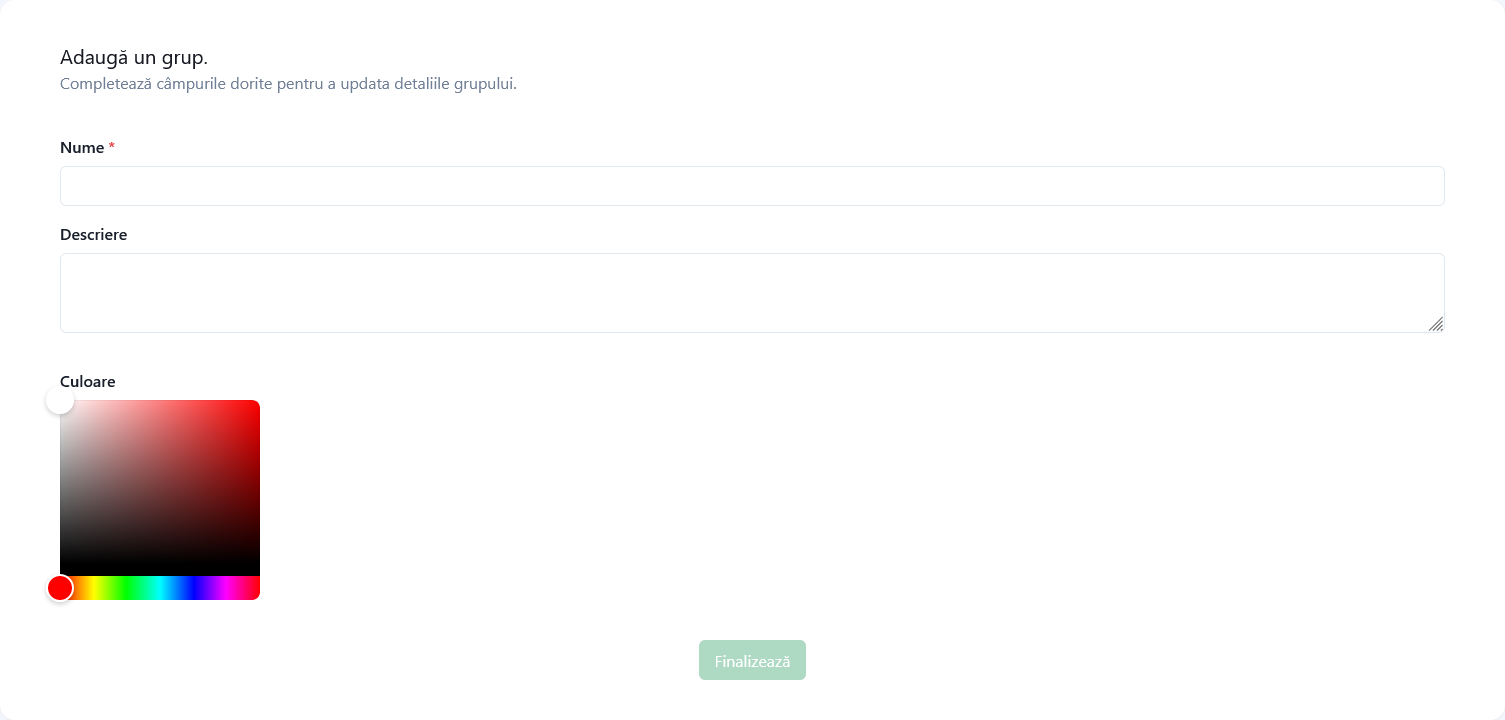
\includegraphics[width=140mm]{images/crud_group.png}
    \caption{Formularul pentru crearea unui grup}
\end{figure}

De asemenea, aplicația Voting App oferă și un strat de securitate în plus în ceea ce înseamnă modificarea datelor în timpul unui proces electoral activ. Platforma nu permite crearea, editarea, sau ștergerea atât a grupurilor, cât și a utilizatorilor  în timpul unui proces electoral deschis, dat fiind că acest lucru ar interveni în validitatea votului și implicit, în necesitatea atingerii cvorumului. În cazul în care administratorul dorește să efectueze schimbări asupra acestor modele, va trebui să închidă orice proces deschis, altfel va fi întâmpinat de o notificare cum că acțiunea pe care dorește să o facă este invalidă.

\newpage

